\documentclass[10pt,a4paper]{article}
\usepackage[utf8]{inputenc}

\usepackage{amsmath}
\usepackage{amsfonts}
\usepackage{amssymb}
\usepackage{graphicx}
\usepackage{listings}

\lstset{numbers=left,
	title=\lstname,
	numberstyle=\tiny,
	breaklines=true,
	tabsize=4,
	language=Python,
	morekeywords={with,super,as},,
	frame=single,
	basicstyle=\footnotesize\tt,
	commentstyle=\color{comment},
	keywordstyle=\color{keyword},
	stringstyle=\color{string},
	backgroundcolor=\color{background},
	showstringspaces=false,
	numbers=left,
	numbersep=5pt,
	literate=
		{�}{{\ae}}1
		{�}{{\aa}}1
		{�}{{\o}}1
		{�}{{\AE}}1
		{�}{{\AA}}1
		{�}{{\O}}1
	}
\usepackage{setspace}
\doublespacing
\usepackage{bm}
\usepackage{hyperref}

\begin{document}
\begin{center}
{\LARGE\bf
FYS4150\\
Project 2, deadline October 2.
}
 
\includegraphics[scale=0.1]{uio.png}\\
Authors: Robin D. Kifle, Sander W. Losnedahl and Vemund S. Thorkildsen\\
University of Oslo, Autumn 2017

{\LARGE\bf Abstract}
\end{center}
\newpage

\begin{center}
{\LARGE\bf Introduction}
\end{center}
<<<<<<< HEAD
The problem we will deal with in this project is of quantum mechanical nature. As none of the three authors have had any quantum mechanics courses we will focus on the mathematical and numerical side of this problem. In this project we are going to develop our own eigenvalue-solver by using Jacobi's method. We will study two different cases, the first is for one electron moving in a harmonic oscillator. The second case is for two electrons moving in a harmonic oscillator with and without repulsive coulomb interaction.
=======
The problem we will deal with in this project is of quantum mechanical nature. As none of the three authors have had any quantum mechanics courses we will focus on the mathematical and numerical side of this problem. In this project we are going to develop our own eigenvalue-solver by using Jacobi's method. We will study two different cases, the first is for one electron moving in a harmonic oscillator. The second case is for two electrons moving in a harmonic oscillator with and without repulsive coulomb interaction. The code, and benchmarks can be found at \url{https://github.com/VemundStenbekkThorkildsen/Assigment2} \\

\noindent The article will start by tackling the mathematics and programming, i.e how the code was made and the mathematics behind it. We will then move on to the results, and discuss these to the best of our ability.  


>>>>>>> 58bbce0acaad76051e3851e1bdbd5c50b02f9403
\newpage

\begin{center}
{\LARGE\bf Method}
\end{center}
To create our eigenvalue solver we first have to take a look at the matrix at hand, to get an understanding of the problem.

$$
  -\frac{d^2}{d\rho^2} u(\rho) + \rho^2u(\rho)  = \lambda u(\rho) .
$$

\noindent This equation will be solved numerically, and has given eigenvalues $\lambda_0=3$, $\lambda_1=7$ and $\lambda_2=11$. We can use the expression for the second derivative to rewrite this. This expression is in our case given by:

$$
 u''=\frac{u(\rho+h) -2u(\rho) +u(\rho-h)}{h^2} +O(h^2)
$$
\noindent
The last part of this expression, namely $O(h^2$, is the truncation error and will not be used further. By using the first part, our expression now looks like this:

$$
\frac{-u(\rho_i+h) +2u(\rho_i) -u(\rho_i-h)}{h^2}+\rho_i^2u(\rho_i)  = \lambda u(\rho_i)
$$

$$
\frac{-u_{i+1} +2u_i -u_{i-1}}{h^2}+\rho_i^2u_i= \lambda u_i
$$

\noindent Our $h$ is given by $h=\frac{\rho_n - \rho_0}{n}$, as we want our $\rho_i$ to vary with step length $h$. By using this $h$, $\rho_i$ will take the form: $\rho_i = \rho_o + ih$. The oscillator potential is given by $(\rho_i)^2$ and will be denoted as $V_i$ in the rest of this article. Now we have everything we need to rearrange this problem as a a matrix eigenvalue problem. \\
\\
From our expression it is easy to see that the matrix we are looking for takes the negative of element $i+1$ and $i-1$, divided by the step length squared. It also need to take two times the positive of element $i$ divided by $h^2$ plus element $i$ multiplied by the oscillator potential $V_i$. This means that we are once again faced by a problem that involves a tridiagonal matrix.

\begin{center}
Main diagonal = $\frac{2}{h^2} + V_i$, first diagonal above and below = $-\frac{1}{h^2}$
\end{center}

\noindent On matrix form this looks like:

\begin{center}


$
 \begin{bmatrix}
 \frac{2}{h^2}+V_1 & -\frac{1}{h^2} & 0   & 0    & \dots  &0     & 0 \\
 -\frac{1}{h^2} & \frac{2}{h^2}+V_2 & -\frac{1}{h^2} & 0    & \dots  &0     &0 \\
  0   & -\frac{1}{h^2} & \frac{2}{h^2}+V_3 & -\frac{1}{h^2}  &0       &\dots & 0\\
  \dots  & \dots & \dots & \dots  &\dots      &\dots & \dots\\
  0   & \dots & \dots & \dots  &\dots  &\dots & \dots\\
 0   & \dots & \dots & \dots  &\dots       & \dots & \frac{2}{h^2}+V_{N-1}
             \end{bmatrix}
             \begin{bmatrix}
             u_0\\
             u_1\\
             u_2\\
             \dots\\
             \dots\\
             u_n\\
             \end{bmatrix} =\lambda
             \begin{bmatrix}
              u_0\\
             u_1\\
             u_2\\
             \dots\\
             \dots\\
             u_n\\
             \end{bmatrix}
$
\end{center}
We are going to solve this by using a Jacobi rotation algorithm. This uses a lot of similarity transformations. As long as:
$$v_j^Tv_i=\delta_{i j}$$
$$U^TU=I$$
The transformations can be shown to preserve the dot product and orthogonality by multiplying with the transpose of the matrix:
$$w=Uv$$
$$w^Tw=(Uv)^TUv=v^TU^TUv=v^Tv=\delta_{i j}$$

<<<<<<< HEAD
\noindent For a symmetric matrix A and Givens rotation matrix R:
=======
\noindent As stated earlier in this article we are going to solve this problem by using the Jacobi eigenvalue algorithm. Consider a symmetric matrix A and Givens rotation matrix R:
>>>>>>> 58bbce0acaad76051e3851e1bdbd5c50b02f9403
$$A'=RAR^T$$
$A'$ is symmetric and similar. $A'$ has entries:
$$A'_{ii} = c^2A_{ii}-2scA_{ij}+s^2A{jj}$$
$$A'_{jj} = s^2A_{ii}+2scA_{ij}+c^2A_{jj}$$
$$A'_{ij} = A'_{ji} = (c^2-s^2)A_{ij}+sc(A_{ii}-A_{jj})$$
$$A'_{ik}=A'_{ki}=cA_ik-sA_{jk} \hspace{3cm} k\neq i,j$$
$$A'_{jk} = A'_{kj} = sA_{ik}+cA_{jk} \hspace{3cm} k\neq i,j$$
$$A'_{kl} = S_{kl} \hspace{5cm} k,l \neq i,j$$
where $s=sin(\theta)$ and $c=cos(\theta)$
We choose $\theta$ such that $A'_{ij}=0$
Rewrite the 3rd equation:
$$A'_{ij}=c(2\theta)A_{ij}+\frac{1}{2}s(2\theta)(A_{ii}-A_{jj})$$
And set this equal to zero:
<<<<<<< HEAD
$$t(2\theta)=\frac{2A_{ij}}{A_{jj}-A_{ii}}$$
if $A_{jj}=A_{ii}$, then $\theta=\frac{\pi}{4}$
This is optimized by using the off-diagonal element with the largest absolute value as $A_{ij}$
The Jacobi eigenvalue method repeats this rotation until the matrix becomes close to diagonal. The elements on the diagonal are then approximations of the real eigenvalues of $A$.
=======
$$tan(2\theta)=\frac{2A_{ij}}{A_{jj}-A_{ii}}$$
if $A_{jj}=A_{ii}$, then $\theta=\frac{\pi}{4}$
This is optimized by using the off-diagonal element with the largest absolute value as $A_{ij}$
The Jacobi eigenvalue method repeats this rotation until the matrix becomes close to diagonal. In reality it checks if all the non-diagonal elements are smaller than a given tolerance. The elements on the diagonal are then approximations of the real eigenvalues of $A$.\\


\noindent The Jacobi eigenvalue method repeats this rotation until the matrix becomes close to diagonal. The elements on the diagonal are then approximations of the real eigenvalues of $A$.


\noindent The algorithm was developed by first creating a matrix $A$ as shown above, letting the matrix size n run from 40 to 400 in 10 steps so that the three lowest eigenvalues produced by a later algorithm would approach 3, 7 and 11 with increasing n.
The first algorithm/function $(maxoffdiag.cpp)$ finds the maximum values of the upper triangular matrix of $A$ and then located the $k$ and $l$ coordinates. The max value of the upper triangular matrix is returned.

\noindent The Jacobi rotation is defined as a function in our script, $rotate.cpp$, and is later called upon in the $jacobi.cpp$. In this script, the matrix is rotated by and angle $\theta$ until the maximum value of the upper, and also the lower diagonal, has a lower value than a set tolerance $\epsilon$ of $10^{-8}$. When all the elements of besides the diagonal is less than $\epsilon$, the rotation stops and the number of iterations is printed for the user to see. 

\noindent The last script $lowesteigen.cpp$ finds the three lowest eigenvalues with the corresponding eigenvectors. The eigenvalues and eigenvectors were saved as a txt file and implemented into a MatLab script to plot.

\noindent Two tests were implemented using user input. The first one is testing if the rotation matrix R is orthogonal so that $R^{T}R = I$. This was calculated by approximately comparing $R^{T}R$ to I. The second test was comparing the numerically calculated eigenvalues of a matrix S to known eigenvalues. If these are approximately the same, then the test passes.
>>>>>>> 58bbce0acaad76051e3851e1bdbd5c50b02f9403


\newpage

\begin{center}
{\LARGE\bf Results}
\end{center}
We have run our algorithm for different cases and focused on different parameters. The different cases have been for two electrons with and without repulsive coulomb interaction. In the first four figures we have focused on the eigenvalues created by the eigenvalue solver. This has been plotted against the number of iterations $n$ for 4 different values of ${\rho}_{max}$. This is compared to the known values of the three lowest eigenvalues, $\lambda_1=3$, $\lambda_2=7$, $\lambda_3=11$, to find a sensible value of ${\rho}_{max}$. In Figure 1 through 7, the potential is set to $\rho^2$

\begin{center}
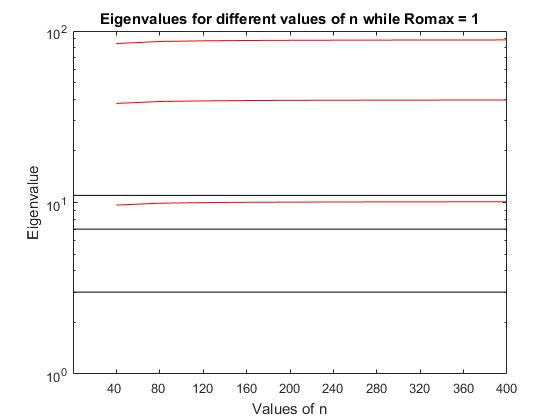
\includegraphics[scale=0.65]{rho1.jpg}

$Figure-1$: Here we have chosen ${\rho}_{max}$ to be 1. As the three lowest eigenvalues are known, this is obviously not a good fit.   



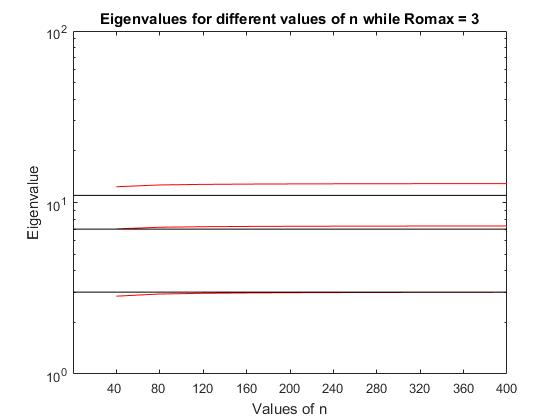
\includegraphics[scale=0.55]{rho3.jpg}

$Figure-2$: Here we have chosen ${\rho}_{max}$ to be 3. The eigenvalues are much closer than in figure 1, but they are still not correct. 


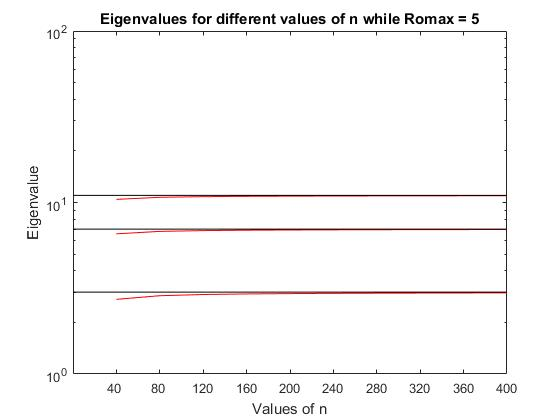
\includegraphics[scale=0.55]{rho5.jpg}
$Figure-3$: Here we have chosen ${\rho}_{max}$ to be 5. In this case all the eigenvalues converge to the correct values. 

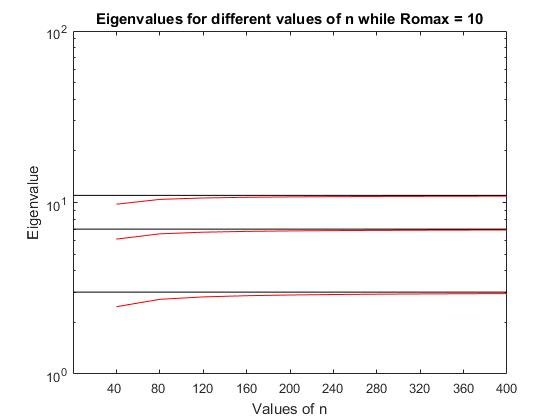
\includegraphics[scale=0.6]{rho10.jpg}
$Figure-4$: Here we have chosen ${\rho}_{max}$ to be 10. In this case all the eigenvalues converge to the correct values, but slower than in the case with ${\rho}_{max}=5$
\end{center}

\noindent From these plots it is easy to see that ${\rho}_{max}=1$ and ${\rho}_{max}=3$ is too low( Figure 1, Figure 2), while the two larger values seem to produce the correct results (Figure 3, Figure 4). The reason for this will be discussed later in the article. Now we can plot the wave functions produced by the same runs, i.e the case with 2 non-interacting electrons. 
\newpage
\begin{center}
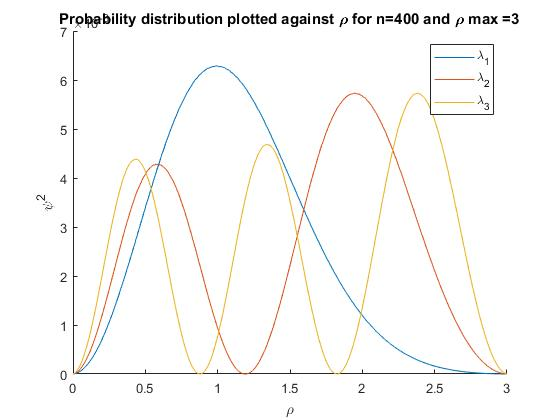
\includegraphics[scale=0.55]{eig400rho3.jpg}
$Figure-5$: Here we have chosen ${\rho}_{max}$ to be 3. The probability distribution is pushed into the boundaries of $\rho$
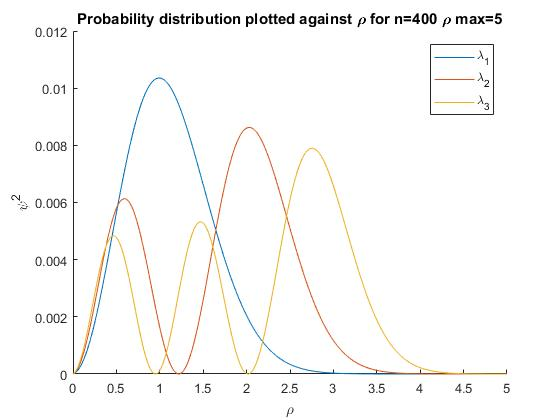
\includegraphics[scale=0.55]{eig400rho5.jpg}
$Figure-6$: Here we have chosen ${\rho}_{max}$ to be 5. The probability dies out before we reach ${\rho}_{max}$. We also see that $\lambda_1$ only has one top, $\lambda_2$ has two tops and $\lambda_3$ has three tops. 

\includegraphics[scale=0.55]{eig360Rho10.jpg}
$Figure-7$: Here we have chosen ${\rho}_{max}$ to be 10. The wave function is of similar shape, and dies out at the approximately the same place as for ${\rho}_{max}=5$. 
\end{center}

\noindent As the wave function dies out at approximately the same place in both Figure 6 and Figure 7, the most sensible ${\rho}_{max}$ will be 5. \\

\noindent One of the problems with the jacobi eigenvalue solver is that it uses a lot of flops, which can take a lot of time. Figure 8 demonstrates that the total number of operations grows exponentially. 
\begin{center}
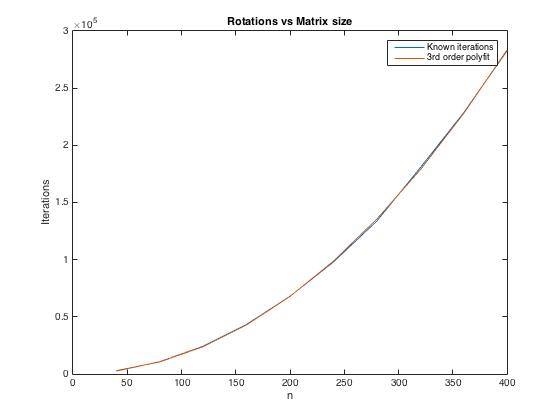
\includegraphics[scale=0.6]{itvsmatsize.jpg}
$Figure-8$: This figure is showing the number of iterations plotted against n. The growth was calculated to be the second order polynomial $1.9x^2-46.5x+2219.3$
\end{center}

\noindent Figure 8 is showing an exponential growth of iterations for growing $n$. This means that the time needed to compute is getting extremely high for high $n$.\\

\noindent In the following figures, the potential is no longer determined by $\rho^2$, it is instead set to ${\omega_r}^2\rho^2 + \frac{1}{\rho}$. We will hold $\rho_{max}$ constant equal to 5 and vary 

\begin{center}
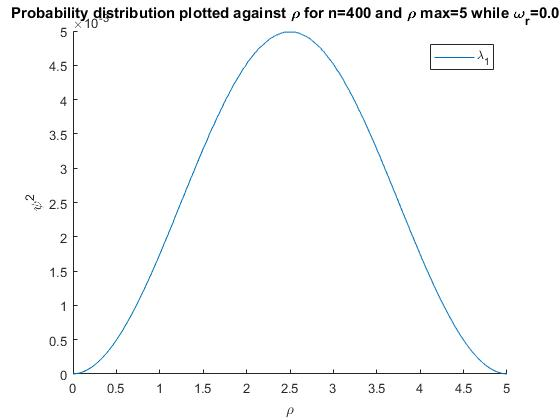
\includegraphics[scale=0.6]{eigomg0011.jpg}
$Figure-9$: The probability distribution for the ground state with $\omega_r=0.01$ is elongated because of the weak potential.   
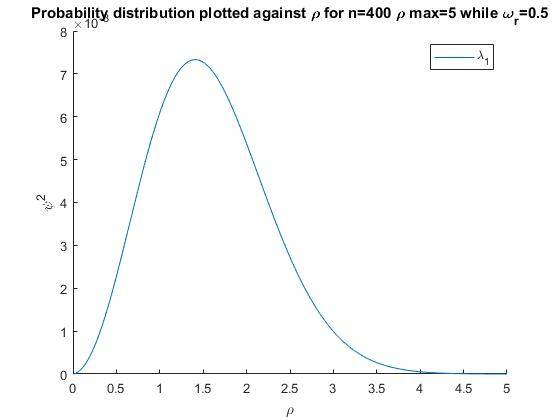
\includegraphics[scale=0.6]{eigomg055.jpg}
$Figure-10$: The probability distribution for the ground state with $\omega_r=0.5$
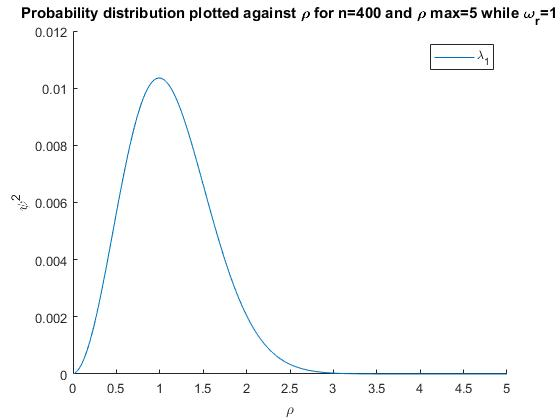
\includegraphics[scale=0.6]{eigomg11.jpg}
$Figure-11$: The probability distribution for the ground state with $\omega_r=1$
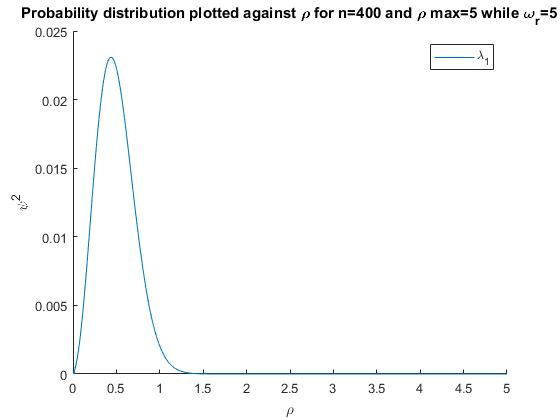
\includegraphics[scale=0.6]{eigomg55.jpg}
$Figure-12$: The probability distribution for the ground state with $\omega_r=5$
\end{center}
For bigger values of $\omega_r$ the probability distribution is shifted to the left
\newpage

\begin{center}
{\LARGE\bf Discussion}
\end{center}

\noindent In the first case we established a sensible value of ${\rho}_{max}$. We were given the analytic solution for the three lowest eigenvalues. By looking at Figure 1,2,3 and 4, it soon becomes clear that using ${\rho}_{max}<5$ does not give the correct eigenvalues. Figure 5 shows this problem in another context. We are effectively trying to push our probability distribution into the boundaries of $\rho$. In figure 6 and 7 we see that the probability dies out before reaching ${\rho}_{max}$. The probability is getting lower for larger $\rho$ but never goes completely down to zero. On these figures we are looking at three different energy levels, corresponding to the three eigenvectors made by the three lowest eigenvalues. It is also possible to see that the probability distributions corresponding to $\lambda_2$ and $\lambda_3$ naturally dies out at respectively $\rho \approx 3.6$ and $\rho \approx 4.5$. If we choose a ${\rho}_{max}$ smaller than this we are, as stated earlier, pushing our probability distribution in to boundaries that are that are too small. This leads to the wrong eigenvalues shown in Figure 1 and 2.\\ 

\noindent As stated earlier in this article, the Jacobi eigenvalue solver is extremely inefficient. Even though we have not timed the algorithm, Figure 8 describes the inefficiency-problem. There is an exponential growth of iterations, and this also effects the execution time. Running the program for $n=400$ can easily take 20 minutes. Running for $n=900$ took us 5 hours. The reason for this extremely long calculation time is that the algorithm checks every non-diagonal to check if it is lower than the given tolerance. In our case $\epsilon=1+^{-8}$\\

\noindent For the second case with two electrons, we ran the program for different values of $\omega_r$. $\omega_r$ reflects the strength of the oscillator potential. Remember that the potential in this case is ${\omega_r}^2\rho^2 + \frac{1}{\rho}$. For weak potential the probability is elongated, that means that the probability of finding the interacting electrons is spread out over a bigger area (Figure 9). By looking at Figure 10 through 12 with increasing potential, it becomes clear that a stronger potential increases the probability of finding the electrons in a narrow window. 




\newpage
\begin{center}
{\LARGE\bf Concluding remarks}
\end{center}
<<<<<<< HEAD
\end{document}
=======
The Jacobi eigenvalue solver we have developed is extremely inefficient. It uses long time to calculate the eigenvalues, because it checks if every non-diagonal element is smaller than the tolerance. By studying the case with two non-interacting electrons, and varying $\rho_{max}$, we found that the eigenvalues were severely altered if $\rho_{max}<5$. With small values of $\rho_{max}$ we are effectively confining the wave function ($\psi$) and probability distribution($\psi^2$) into a too small area. This is altering the wave function and probability distribution. In the case with two electrons interacting, we studied the effect of varying potential strength. The algorithm is the same in both cases, but the potential is different. For cases with weak potential the probability is widespread. With stronger potential, the probability is shifted to $\rho_0=0$ and narrows. 
\newpage
\begin{center}
{\LARGE\bf References}
\noindent Jensen, M.H. (2015). Computational Physics, Lecture Notes Fall 2015 [Online lecture notes]. Retrieved from https://github.com/CompPhysics/ComputationalPhysics/blob/master/doc/Lectures/lectures2015.pdf
\end{center}
\end{document}
>>>>>>> 58bbce0acaad76051e3851e1bdbd5c50b02f9403
